
\begin{figure}
\centering
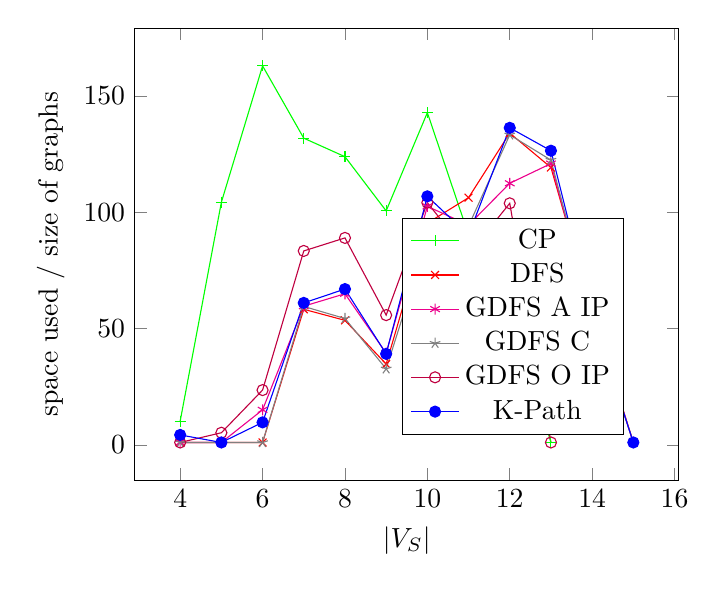
\begin{tikzpicture}
    \begin{axis}[
        xlabel=$|V_S|$,
        ylabel=space used $/$ size of graphs,
        legend style={at={(0.9,0.1)},anchor=south east},
        width=0.7\textwidth,
		%y tick label style={/pgf/number format/sci},
    ]

%    \node[] at (axis cs: 9,1.1) {Awaiting test results (CAES server)};

\addplot[
        mark=+,
        green,
    ] plot coordinates {
        (4,10.174505370550349224253838)
        (5,104.28268407548150313423625)
        (6,162.90001905722773387141976)
        (7,131.82092679714642689897069)
        (8,123.86131153662219616440982)
        (9,100.54876902079979411614113)
        (10,142.8055123071906161809092)
        (11,90.23704183358028315864566)
        (12,60.13828770787494509749228)
        (13,1)
};
    \addlegendentry{CP}
    
    \addplot[
        mark=x,
        red,
    ] plot coordinates {
        (4,1)
        (5,1)
        (6,1)
        (7,58.25769782075416109734502296)
        (8,53.49977853854609387401796491)
        (9,34.69315781105574763597362315)
        (10,95.2821470489074655940527300)
        (11,106.247669775327306151566700)
        (12,134.009989654390014925155652)
        (13,119.208253326512152230628507)
        (14,57.5163619146955535818220329)
        (15,1)
};
    \addlegendentry{DFS}

    \addplot[
        mark=asterisk,
        magenta,
    ] plot coordinates {
        (4,1)
        (5,1)
        (6,15.02985034471161930)
        (7,59.59097376035428638)
        (8,64.93368304714666954)
        (9,39.37678578646825642)
        (10,102.493087611314720)
        (11,94.4701670636009438)
        (12,112.425234638110666)
        (13,120.892092891415954)
        (14,56.0582514421801884)
        (15,1)
};
    \addlegendentry{GDFS A IP}
    
    \addplot[
        mark=star,
        gray,
    ] plot coordinates {
        (4,1)
        (5,1)
        (6,1)
        (7,59.479189954442690)
        (8,54.294753873478837)
        (9,32.656874607567579)
        (10,88.62263521222060)
        (11,94.07313175657136)
        (12,133.2439360650590)
        (13,122.4129802403613)
        (14,55.53333167207465)
        (15,1)
};
    \addlegendentry{GDFS C}
    
    \addplot[
        mark=o,
        purple,
    ] plot coordinates {
        (4,1)
        (5,5.1826054759816817)
        (6,23.512962277899220)
        (7,83.341983867316274)
        (8,88.941938162115534)
        (9,55.750056887542679)
        (10,104.1015790897492)
        (11,81.84559512703726)
        (12,103.8155851653250)
        (13,1)
};
    \addlegendentry{GDFS O IP}
    
    \addplot[
        mark=*,
        blue,
    ] plot coordinates {
        (4,4.240778515784331992)
        (5,1)
        (6,9.641524578218709713)
        (7,61.00961187901417579)
        (8,66.94762056230962072)
        (9,39.09244788901674288)
        (10,106.812982924035309)
        (11,90.1677790988596005)
        (12,136.268506857638343)
        (13,126.432468234002608)
        (14,55.5333316720746569)
        (15,1)
};
    \addlegendentry{K-Path}
	
    \end{axis}
    \end{tikzpicture}
    \caption{Space usage of the algorithm with each path iterator relative to the space usage of the input graphs. Unnecessarily long paths are avoided, target vertices are ordered by degree and contraction is disabled.}
    \label{fig:spaceusage-pathiterators}

\end{figure}
